% !TeX root = ../main.tex

\chapter{基于深度学习的时间序列异常检测框架设计与实现}
\label{cha:anomaly:detection}
本章主要介绍本文实现的基于深度学习的时间序列异常检测框架,对执行流程和各个部分的设计进行详细说明。
\section{形式化定义}
首先我们形式化地描述一下时间序列异常检测问题。一个时间序列是等时间间隔收集到的各个指标的值,定义为$x=\{x_1,x_2,\dots,x_N\}$,$N$是采集的次数。由于本文考虑的是多元时间序列的异常检测,所以每个时间都会有多个监测指标的值,也就是其中$x_t\in R^M$,$x_t=[x_t^1,x_t^2,\dots,x_t^M]$,其中$t\leq N$,$M$是数据的维度。所以$x\in R^{N\times M}$。我们最终目标是输出一个$y=[y_1, y_2,\dots, y_N ]$,其中$y_t\in \{0,1\}$,$y_t=0$代表该时刻检测到的指标正常,否则认为发现一个异常。图\ref{fig:anomaly_example}展示了一个异常示例,其中标红部分为一个出现异常的事件段。
\begin{figure}[htbp]
  \centering
  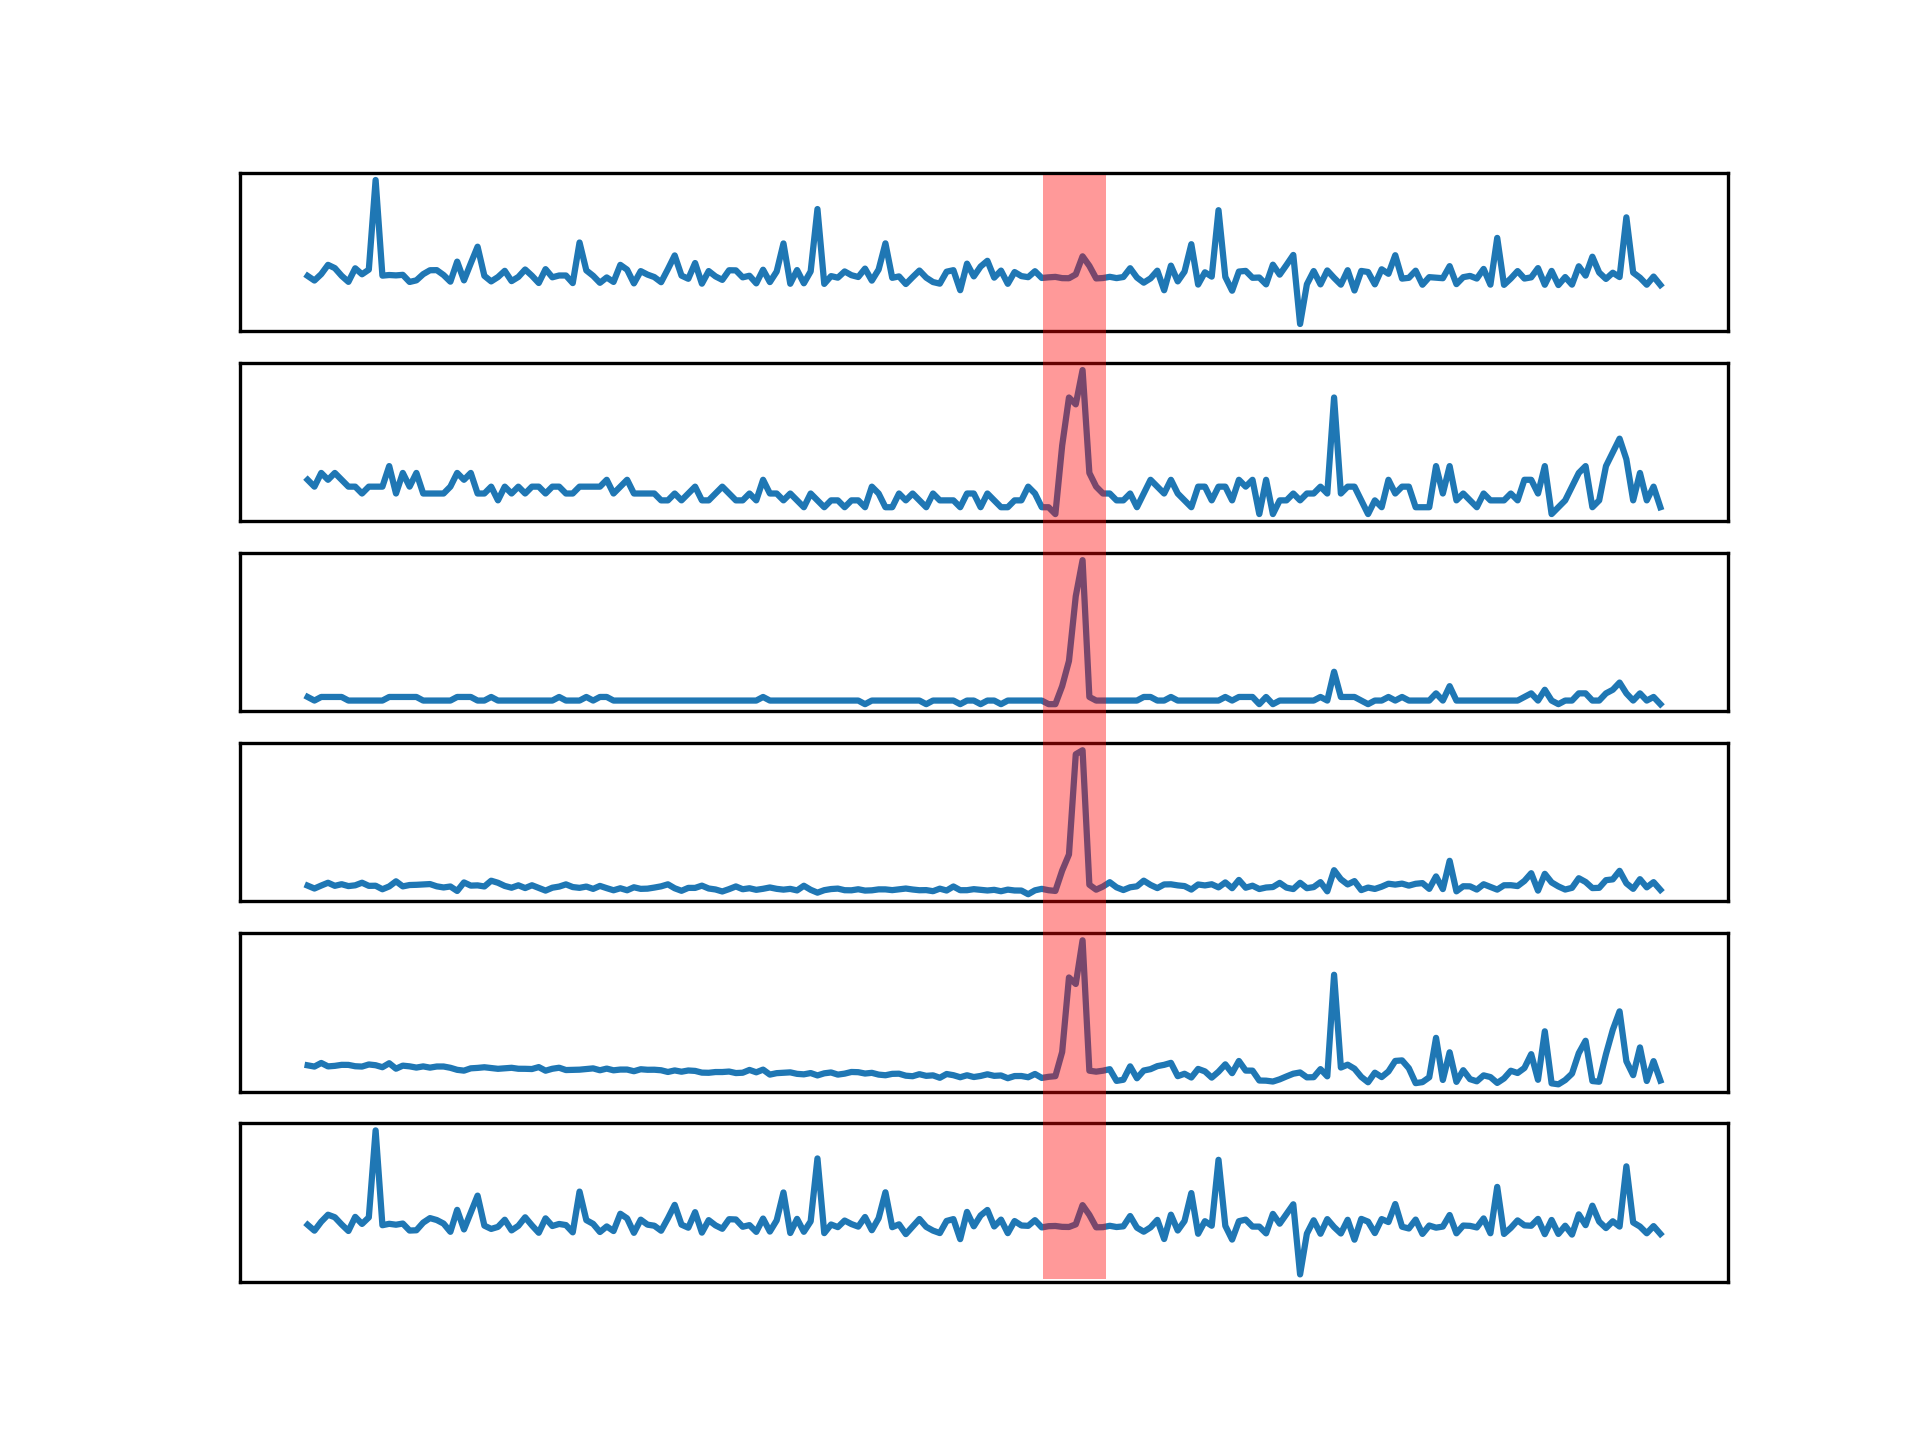
\includegraphics[width=\textwidth]{another_anomaly_example.png}
  \caption{多维时间序列数据中的一个异常示例}
  \label{fig:anomaly_example}
\end{figure}

\section{框架设计}
本文实现的基于深度学习的时间序列异常检测框架如图~\ref{fig:part1_overview}所示

\begin{figure}[htbp]
    \centering
    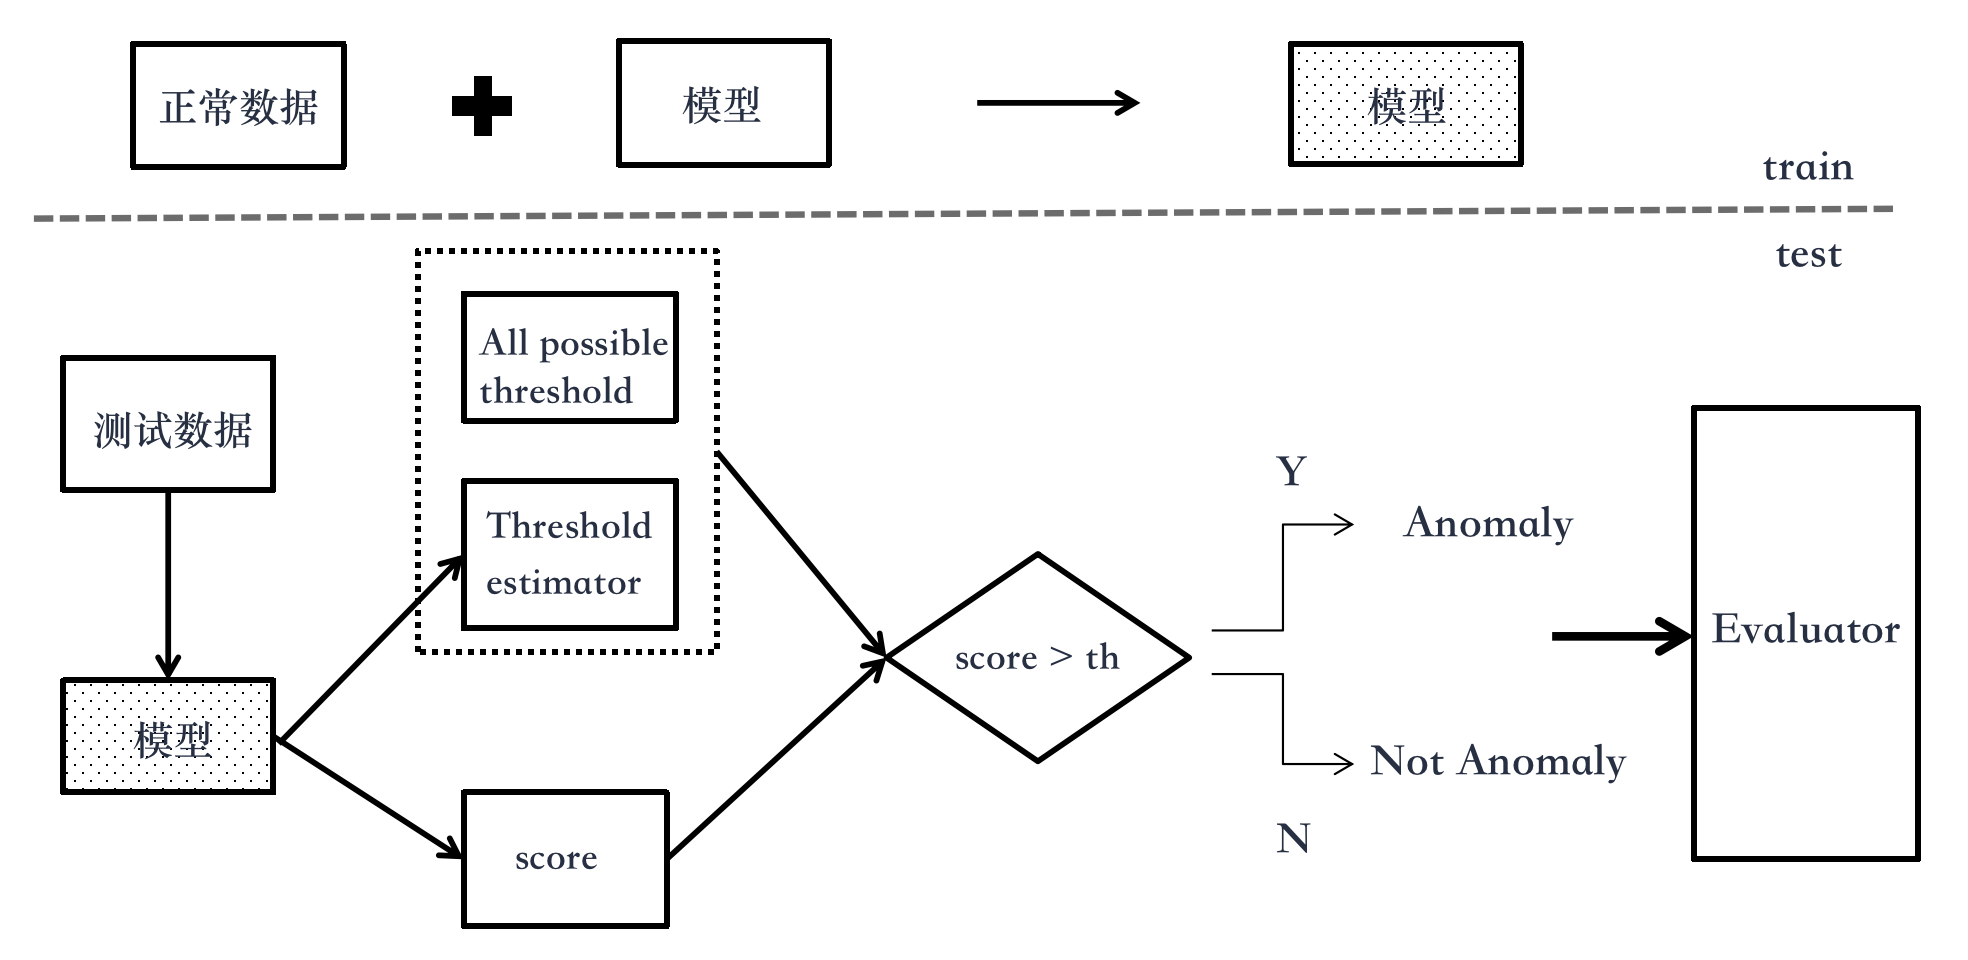
\includegraphics[width=\textwidth]{part1_overview.png}
    \caption{基于深度学习的时间序列异常检测框架}
    \label{fig:part1_overview}
  \end{figure}

本文涉及的框架分为训练和测试两个步骤。

在训练时,需要先用正常数据结合某个特定的模型训练出一个适用于该数据集的模型。然后在测试时,模型对于每一时刻会输出一个异常分数通常为非负实数表示此时的异常程度,值越大表示越异常,但由于最终输出的是一个是否是异常的01值,所以通常情况下还需要模型来提供一个阈值,当异常程度>给定阈值时,认为该条数据是异常,否则认为正常,然后将得到的预测结果送到评估模块与真实的异常标签进行结果的评估。由于阈值的确立有多种方法,每个算法适用的确立阈值的方法的也不尽相同,因此本文还同时枚举所有可能的阈值对结果进行评估,选取结果最好的来衡量模型的上限\cite{xu2018unsupervised,su2019robust,DBLP:conf/ipccc/LiCP18,DBLP:conf/infocom/ChenXLPCQFW19}。

接下来分别对框架的几个关键部分进行阐述
\section{数据集选择}
目前用来做多维时间序列数据异常检测的数据集如表~\ref{tab:dataset}所示:

\begin{table}[htbp]
  \centering
  \begin{tabular}{lcccc}
    \toprule
    名称 & 类型 & 单点数量 & 指标数量  & 指标名称 \\
    \midrule
    SMD\cite{su2019robust} & 服务器数据 & 28 & 38 & CPU利用率,网络吞吐量等\\
    SMAP\cite{DBLP:conf/kdd/HundmanCLCS18} & \multirow{2}{*}{飞船监测数据} & 55 & 25 & \multirow{2}{*}{辐射,温度,功率等}\\
    MSL\cite{DBLP:conf/kdd/HundmanCLCS18} &  & 27 & 55 &  \\
    Robot\cite{park2018multimodal} & 机器人传感数据 & \approx 39 & 17 & 运动,视觉,听觉,触觉等\\
    Engine\cite{malhotra2016lstm} &工业机器监测数据 & - & 12 & 加速器,扭矩,温度等\\
    \bottomrule
  \end{tabular}
  \caption{多元时间序列数据异常检测的数据集\cite{su2019robust}}
  \label{tab:dataset}
\end{table}

考虑到场景的类似性,我们选择了在SMD\cite{su2019robust}数据集上完成实验。其是从国内某互联网公司的服务器上采集的真实数据进行脱敏处理后的结果。测量了28台机器上的38个指标长达5周的结果,也就是$M=38$,每个机器上都采集了等间隔的超过40000个等时间间隔的数据,然后将数据平均分为了两部分,一部分全是正常数据$x_{train}$,其中不包含异常,而另一部分则包含异常$x_{test}$并且提供了标记$y_{test}$用来测试。

\section{算法选择模块}
在算法的选择方面,本文实现了两部分的算法,一部分是复现一些经典的算法,另一部分则是对已有算法进行一些修改来适应于当前的问题。
\subsection{复现算法}
本文复现了一些经典的异常检测算法,主要包含两类,一类是用于单点异常检测的算法,即将每个时间点的数据当成独立不相关的数据进行检测,也就是将这些模型看做一个函数的话,就是$y_t = \phi (x_t)$,例如AutoEncoder、Variational AutoEncoder\cite{an2015variational}、Deep SVDD\cite{ruff2018deep}、DAGMM\cite{zong2018deep}、ConAD\cite{nguyen2018anomaly};另一类则是判断每一时刻的状态时不仅要看当前的指标监测值,还要看之前一段时间数据,不妨令这段时间长度为$T$,则$y_t = \phi(x_{t-T},x_{t-T+1},\dots,x_{t})$,具体LSTM、LSTM-ED\cite{malhotra2016lstm}。
\subsection{改进算法}
在已有算法的基础上,我们做出了两方面的改进。

一方面是修改已有的用于单点异常检测的算法结构来使其适应时间序列异常检测,将原来的单点方法与时序模型例如LSTM结合起来捕捉时间上的依赖信息,具体做法是将原算法中的Linear层替换成LSTM层来保留和捕捉历史信息,比方说对AutoEncoder的模型改变如图~\ref{fig:lstm_ae}所示。依据此种方法,我们还对VAE、ConAD进行修改分别得到了LSTM-VAE和LSTM-ConAD模型。

\begin{figure}[htbp]
  \begin{minipage}[t]{0.5\linewidth}
  \centering
  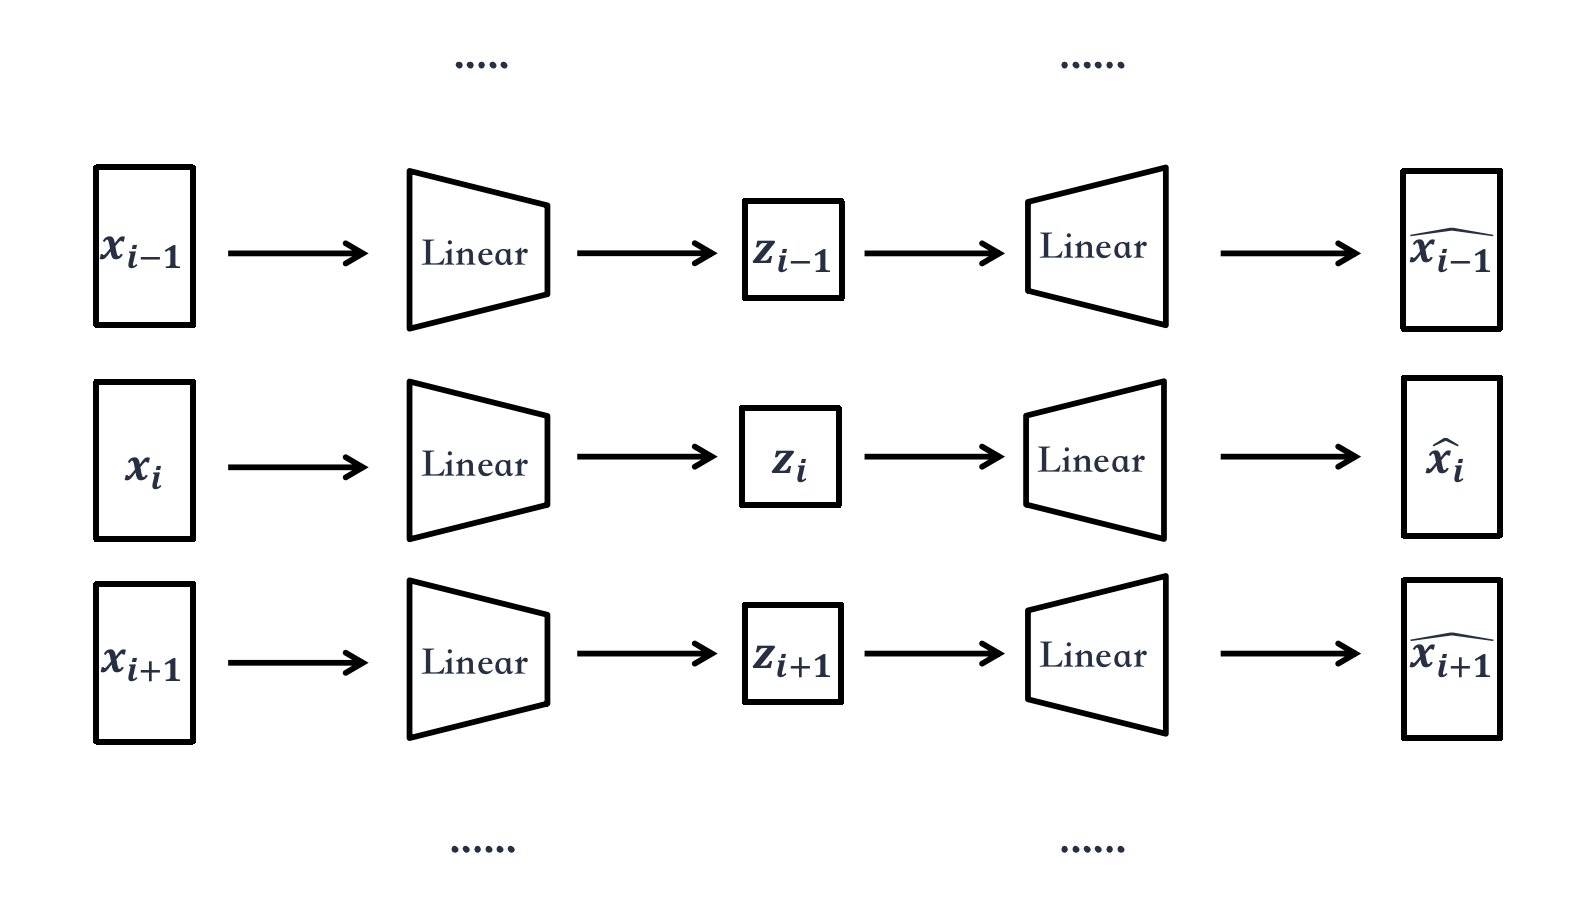
\includegraphics[width=\textwidth]{AE.png}
  \caption*{原先的AutoEncoder模型}
  \end{minipage}
  \begin{minipage}[t]{0.5\linewidth}
  \centering
  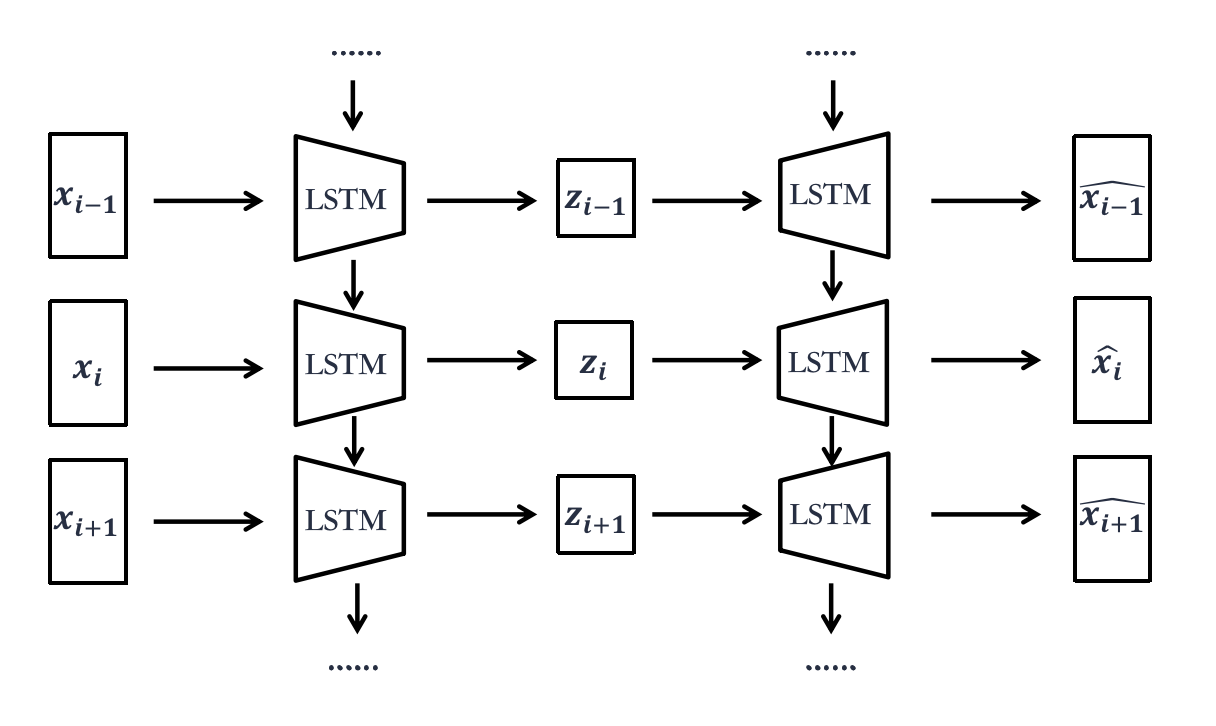
\includegraphics[width=0.95\textwidth]{LSTM_AE.png}
  \caption*{经过修改后的LSTM\_AE模型}
  \end{minipage}
  \caption{对AutoEncoder的模型修改过程}
  \label{fig:lstm_ae}
\end{figure}

另一方面是我们将LSTM的预测与AE的重构结合起来,提出了一个AE-Predictor模型,其结构如图~\ref{fig:AE-Predictor}所示。

\begin{figure}[htbp]
  \centering
  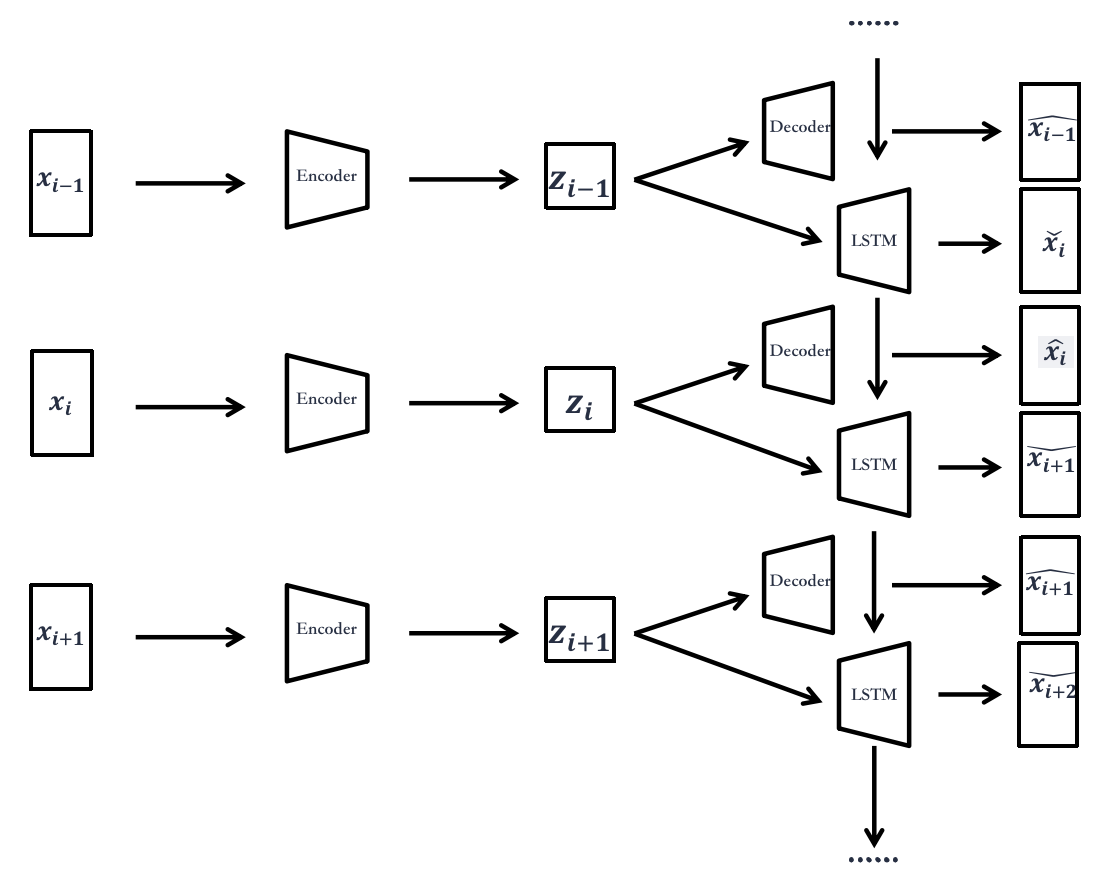
\includegraphics[width=0.7\textwidth]{AE_Predictor.png}
  \caption{AE-Predictor模型示意图}
  \label{fig:AE-Predictor}
\end{figure}

目的是要让AE学习的低维表示不仅具有重构当前数据的能力,同时低维表示序列还具有能够预测下一时刻数据的能力,也就是捕捉到时序依赖,以此达到更好的异常检测效果。

\section{动态阈值选取模块}
因为在算法选择部分均是实现的无监督的算法,因此通常算法输出的是一个异常分数的非负实数值,而不是一个0或者1的确切值,也就是说得到的实际是$s = [s_1, s_2,\dots,s_N]$,其中$s_t\in R^+$,$t\leq N$,要想进一步得到$y$,需要一个模型提供的或者人为提供的阈值$threshold$来作进一步的变换:
\begin{equation*}
  y_t = \begin{cases}
    0, & s_t < threshold \cr
    1, & s_t \geq threshold
  \end{cases}
\end{equation*}

通常情况下,该阈值的确立有多种方法,一种是假设异常分数满足特定分布,例如高斯分布,求出正常数据下的异常分数的均值$\mu$和方差$\sigma$,那么异常分数超过$\mu + 3\sigma$的数据理论上不到0.3\%,那么我们就可以认为异常分数位于这个范围内数据是异常,但实际的异常分数很难从理论上证明符合高斯分布,通常情况下也确实不符合;还有一种比较简单的方式是假设异常是异常分数最高的那一批,通过人为设定一个分位数,例如5\%,那么在测试时就直接将最高的那5\%的数据标为异常,但这个分位数的选取也是个难题,异常的比例事先并不知道,而且,该方法需要知道整个测试集的情况才能确立阈值,意味着只能做离线的异常检测;还有一种方法是通过在验证集上选取合适的阈值以及基于验证集和测试集情况类似的假设来期待在测试集上获得较好的效果,这种方法的缺点在于我们还需要另一份有标数据来进行阈值的确定,在真正落地的时候难度较大。

受到\cite{siffer2017anomaly}的启发,我们使用了极值理论中的POT方法来确立异常分数的阈值,好处是无需对原分布做出任何假设,可以准确、在线地确立阈值。其基本思想就是通过带有参数的GPD\footnote{Generalized Pareto Distribution,广义帕累托分布}来拟合概率分布的尾部:
\begin{equation*}
  \hat{F}_{th}(s) = P(S - th > s | S > th) \approx (1 + \frac{\gamma s}{\beta})^{-\frac{1}{\gamma}}
\end{equation*}

其中$th$是一个异常分数的初始阈值,用来确定尾部区域,可以凭经验地设为正常数据的异常分数的一个较大的分位数,$\gamma$和$\beta$是GPD的形状和比例参数,是两个未知参数,可以用最大似然估计\cite{white1982maximum}的方法得到参数$\hat{\gamma}$和$\hat{\beta}$,然后通过以下公式计算最终阈值$th_F$:
\begin{equation*}
  th_F \approx th + \frac{\hat{\beta}}{\hat{\gamma}}((\frac{qN'}{N_{th}})^{-\hat{\gamma}}-1)
\end{equation*}

其中$q$是观察$S<th_F$的期望概率,也是POT算法的一个输入,可以凭经验确定,$N$是总的数据点个数,$N_{th}$是"尾部"的数据点的个数。

该部分提到的几种方法总结如表~\ref{tab:threshold}所示。


\begin{table}[htbp]
  \centering
  \begin{tabular}{lccc}
    \toprule
    方法 & 假设 & 有标 & 在线 \\
    \midrule
    假设异常分数满足特定分布 & 强 & × & √ \\
    假设异常占一定比例 & 强 & × & × \\
    划分验证集 & 弱 & √ & √ \\
    POT & 弱 & × & √\\
    \bottomrule
   \end{tabular}
   \caption{确立阈值的方法对比}
   \label{tab:threshold}
\end{table}

\section{评价模块}
在异常检测领域,用的最多的评价指标是F\_1-Score,计算方式为
\begin{equation*}
  Precision = \frac{TP}{TP + NP}
\end{equation*}

\begin{equation*}
  Recall = \frac{TP}{TP + FN}
\end{equation*}

\begin{equation*}
  F_1-Score = 2\times \frac { Precision \times Recall}{Precision + Recall}
\end{equation*}

其中$TP$、$TN$、$FP$、$FN$分别代表true positives、true negatives、false positives和 false negatives。$Precision$描绘的是实际异常占检测出的所有异常的比例,而$Recall$描绘了所有的异常中被检测到的比例,直觉上来看,两者是对立的,单用其中一个用来评价检测器的性能是不合理的。但在单点的异常检测中,将它们结合在一起的$F_1-Score$已经被认为是公认的有效的评价方式。但对于时间序列数据的异常检测来说,这样的评价就不太准确。主要原因是因为在时间序列数据中异常的发生通常是连续的一段,如图\ref{fig:anomaly_example}所示。对于一段真正的异常而言,检测到异常的点的个数以及检测出来的位置都反映了模型效果的不同,例如一段长度为10的异常,模型$A$检测到了其中的8个,而模型$B$只检测到了1个,那么相对而言前者的效果会更好;如果模型$A$在这段异常开始的第一个位置就检测到了异常,而模型$B$直到第5个点才检测到,那么在实际投入使用时,前者的效果一定是我们更想要,能够帮助工作人员更早地发现异常。之前的一些工作\cite{xu2018unsupervised}\cite{su2019robust}用了一种point-wise的方法来对算法得到的结果进行调整然后再进行评估,具体就是对于一个真实的异常而言,如果我们的算法主要检测到了范围内的一个,那么整段异常就认为都被检测到。该评价方法没有考虑到检测到的点的位置和检测到的点数的影响,会造成评价指标的虚高。

基于以上考虑,本文借用了\cite{tatbul2018precision}的新型的Precision和Recall的计算方式。

首先将异常表示成区间的集合,真实的异常为$R=[R_1,R_2,\dots,R_{N_r}]$,其中每个$R_i$代表一个区间的异常,不妨认为$R_i.l$和$R_i.r$分别代表该区间的左右端点。同理$P=[P_1,P_2,\dots,P_{N_p}]$表示预测出来的异常。
\begin{equation*}
  Recall(R,P) = \frac{\sum_{i=1}^{N_r} Recall_T(R_i,P)}{N_r}
\end{equation*}

其中$Recall_T$的计算由两部分加权组成:分别考虑了存在性以及位置性。
\begin{equation*}
  Recall_T(R_i,P) = \alpha \times ExistenceReward(R_i,P) + (1-\alpha) \times OverlapReward (R_i,P)
\end{equation*}

存在性只需要判断是否存在一个检测出的异常区间当前的实际异常有交集。
\begin{equation*}
ExistenceReward(R_i,P) = \begin{cases} 1, & \ \exists \  | R_i \cap P_j|>1 \cr 0, & otherwise \end{cases}
\end{equation*}

而相交性则需要考虑重叠的位置和大小的关系,此处本文认为对于一段异常来说,越早检测到说明效果越好,因此将靠前的位置分配较大的权重,具体计算如算法~\ref{algorithm:omega1}所示。
\begin{equation*}
  OverlapReward(R_i,P) = \sum_{j=1}^{N_p}\omega(R_i,R_i\cap P_j)
\end{equation*}
\begin{algorithm}
  \caption{$\omega$ 原版计算方法\cite{tatbul2018precision}}
  \begin{algorithmic}
      \Function{$\omega$}{AnomalyRange, OverlapRange}
      \State DetectValue \gets 0
      \State TotalValue \gets 0
      \State len \gets length(AnomalyRange)
      \For {i = 1  \to len}
          \State Value \gets len - i + 1
          \State TotalValue \gets TotalValue + Value
          \If {AnomalyRange[i] in OverlapRange}
              \State DetectValue \gets DetectValue + Value
          \EndIf
      \EndFor
      \State \Return $\frac{DetectValue}{TotalValue}$
      \EndFunction
  \end{algorithmic}
  \label{algorithm:omega1}
\end{algorithm}

意识到$OverlapRange$也一定是一个区间之后,可以将$\omega$的计算方式简化为算法~\ref{algorithm:omega2}:
  \begin{algorithm}
    \caption{$\omega$ 简化计算方法}
    \begin{algorithmic}
        \Function{$\omega$}{AnomalyRange, OverlapRange}
        \State len \gets length(AnomalyRange)
        \State TotalValue \gets $\frac{len \times (len + 1)}{2}$
        \State l \gets OverlapRange.l - AnomalyRange.l + 1
        \State r \gets OverlapRange.r - AnomalyRange.l + 1
        \State DetectValue \gets $\frac{r \times (r+1)}{2} - \frac{(l-1) \times l}{2}$
        \State \Return $\frac{DetectValue}{TotalValue}$
        \EndFunction
    \end{algorithmic}
    \label{algorithm:omega2}
  \end{algorithm}

新型Precision的计算方式类似:

\begin{equation*}
Precision(R,P) = \frac{\sum_{i=1}^{N_p}Precision_T(R,P_i)}{N_p}
\end{equation*}

区别是$Precision_t(R,P_i)$的计算不需要考虑$ExistenceReward$,直接按照检测到的位置算贡献即可:
\begin{equation*}
Precision_T(R,P_i) = \sum_{j=1}^{N_r}\omega(P_i,P_i\cap R_j)
\end{equation*}

  该评价方式虽然考虑的全面,但是随之而来的就是计算代价很大,复杂度为$O(N_r\times N_p)$。当我们需要计算所有阈值的结果并选取最好的时候,考虑阈值按从大到小枚举所有可能的$N$个,最坏情况下的$N_p$序列为$\{1,2,3,\dots,\frac{N}{2},\frac{N}{2}-1,\frac{N}{2}-2,\dots,1\}$,则总的计算复杂度为$O(N_r\times N^2)$。

  \begin{algorithm}
  \caption{朴素的Best F1-Score计算方式}
  \begin{algorithmic}[1]
    \Function {computeBestF1Score}{R,S}
    \State bestF1Score = 0
    \ForAll {$s \in S$}
    \State P \gets convertTo01ByThreshold(S,s)
    \State bestF1Score \gets max(bestF1Score, computeF1Score(R,P))
    \EndFor
    \State \Return bestF1Score
    \EndFunction
  \end{algorithmic}
  \end{algorithm}


  我们考虑一种新的增量计算的方式,每次将阈值下调时,考虑只有一个位置$i$的预测结果从0变成了1,那么有可能有三种情况:
  \begin{enumerate}
    \item 这一个位置形成了一个新的异常区间,也就是$i-1$和$i+1$都是不存在或者为0的状态
    \item 这个位置拓宽了相邻的区间,也就是$i-1$或者$i+1$中有且只有一个位置已经被预测为1
    \item 这个位置将左右两个区间连成了一个区间,也就是$i-1$与$i+1$都存在且被预测为异常
  \end{enumerate}

  如果我们能够以一个较低的复杂度支持动态的在$P$中增加、减少一个异常区间同时计算$Precision$和$Recall$的值,那么就能高效的求解$Best F1-Score$。具体来讲,我们通过记录中间变量的方式来记录计算过程中的中间状态,通过并查集的方式来快速维护$P$。具体的算法过程如下:

  \begin{breakablealgorithm}
    \caption{高效的Best F1-Score计算方式}
    \begin{algorithmic}[1]
      \State $rangeReward \gets [0] \times N_r$
      \State $rangeOverlapCount \gets [0] \times N_r$
      \State $predict \gets [0] \times N$
      \State $Recall \gets 0$
      \State $Precision \gets 0$

      \State

      \Function {computeBestF1Score}{R,S}
      \State bestF1Score = 0
      \State S \gets sorted(S) in descending order
      \ForAll {$S_i \in S$}
      \State $predict_i = 1$
      \If { $i + 1 < n\ and\ predict_{i+1} = 1$}
          \State \Call{dropPredictRange}{\Call{GetRange}{i + 1}}
          \State \Call{union}{i, i + 1}
      \EndIf
      \If {$i - 1 \geq 0\ and\ predict_{i-1} = 1$}:
          \State \Call{dropPredictRange}{\Call{GetRange}{i - 1}}
          \State \Call{union}{i, i - 1}
      \EndIf
      \State \Call{addPredictRange}{\Call{GetRange}{i}}
      \State $bestF1Score \gets max(bestF1Score, 2\times\frac{Precision \times Recall}{Precision + Recall})$
      \EndFor
      \State \Return bestF1Score
      \EndFunction
      
      \State

      \Function {addPredictRange}{p}
      \State Recall \gets 0
      \ForAll{$R_i \in R$}
            \State $rangeReward_i \gets rangeReward_i + \omega(R_i,R_i \cap p)$
            \State $overlapCount_i \gets overlapCount_i +  |R_i\cap p|$
            \If {$overlapCount_i > 0$}
              \State existReward = 1
            \Else
              \State existReward = 0
            \EndIf
            \State $overlapReward \gets rangeReward_i$
            \State $Recall \gets Recall + \alpha \times existReward + (1-\alpha) \times overlapReward$
      \EndFor
      \State $Recall = \frac{Recall}{N_r}$

      \State

      \State $reward \gets 0$
      \ForAll{$R_i \in R$}
            \State $reward \gets reward  + \omega(p, p \cap R_i)$
      \EndFor
      \State $Precision \gets \frac{Precision \times N_p + reward}{N_p + 1}$
      \State $N_p \gets N_p + 1$
      \EndFunction

      \State

      \Function {dropPredictRange}{p}
      \State Recall \gets 0
      \ForAll $R_i \in R$
            \State $rangeReward_i \gets rangeReward_i - \omega(R_i,R_i \cap p)$
            \State $overlapCount_i \gets overlapCount_i - |R_i\cap p|$
            \If {$overlapCount_i > 0$}
              \State $existReward = 1$
            \Else
              \State $existReward = 0$
            \EndIf
            \State $overlapReward \gets rangeReward_i$
            \State $Recall \gets Recall +  \alpha \times existReward + (1-\alpha) \times overlapReward$
      \EndFor

      \State

      \State $Recall \gets \frac{Recall}{N_r}$

      \State $reward \gets 0$
      \ForAll $R_i \in R$
            \State $reward \gets reward + \omega(p, p \cap R_i)$
      \EndFor
      \State $Precision \gets \frac{Precision \times N_p - reward}{N_p - 1}$
      \State $N_p \gets N_p - 1$
      \EndFunction
    \end{algorithmic}
  \end{breakablealgorithm}

  其中GetRange和Union是通过并查集来实现记录和维护某个位置所属的区间以及该区间的左右端点,算法中不再赘述。容易得知这样的计算复杂度为$O((N_r + \alpha(N))\times N)$,其中$\alpha(N)$是Ackerman函数的某个反函数,在很大一个范围内(超过$10^{80}$)可以认为是不大于4的一个常数,所以我们可以认为复杂度是较原先下降了一个数量级,实测原先需要4小时的计算仅需3秒就可以得出结果。
\section{实验结果与分析}
本章先对所有算法在所有阈值下的最好结果进行分析,再评估用POT方法确立阈值对结果造成的影响及其效率,然后对比一下传统基于点的异常检测模型与时序模型结合后与原模型的效果,最后我们对各个算法的效率进行比较。
\subsection{最好结果}
表~\ref{tab:best}为各个算法在枚举所有阈值之后得到的最好的评估结果,其中Random是随机将当前时刻分为正常或异常,OmniAnomaly是\cite{su2019robust}中提出的模型,在我们的框架内并没有实现,我们使用其公开的源代码进行了异常检测的结果获取然后放到我们的评估模块中进行评估,方便参考。
\begin{table}
  \centering
\begin{tabular}{lccc}
  \toprule
          algorithm &  F1-Score &    Recall &  Precision \\
  \midrule
   LSTM-VAE &  0.779323 &  0.708920 &   0.865252 \\
        VAE &  0.768701 &  0.718729 &   0.826141 \\
     LSTM &  0.740222 &  0.712757 &   0.769889 \\
            LSTM-AE &  0.736745 &  0.694566 &   0.784377 \\
       AE-Preditor &  0.723190 &  0.690104 &   0.759609 \\
                 AE &  0.715418 &  0.687829 &   0.745311 \\
                 OmniAnomaly &  0.708538 &  0.662548 &   0.761388 \\
         LSTM-ConAD &  0.666084 &  0.648798 &   0.684316 \\
              ConAD &  0.655414 &  0.613009 &   0.704121 \\
          Deep SVDD &  0.585766 &  0.606182 &   0.566680 \\
            LSTM-ED &  0.582350 &  0.567344 &   0.598172 \\
              DAGMM &  0.568452 &  0.721212 &   0.469093 \\
             Random &  0.177244 &  0.813319 &   0.099459 \\
  \bottomrule
  \end{tabular}
  \caption{各个算法的枚举所有阈值选取最好的评估结果}
  \label{tab:best}
\end{table}

从表中可以看出:
\begin{itemize}
  \item 重构和预测的方法都取得了不错的效果,这其中又属将重构和预测结合起来的LSTM-VAE表现最好;
  \item ConAD模型表现并不佳,很可能是数据分布并不符合多假设分布,所以直接套用效果并不好;
  \item OmniAnomaly在自己的评价标准中是最好的,但在我们的框架中表现并不突出。从方法上来看,我们偏向于认为我们的评价方式更有说服力;
  \item 我们提出的AE-Predictor比AE的结果稍好,但仍然不如纯用LSTM的结果,可见其能捕捉到的时序特征有限;
  \item 不论是VAE和AE,还是LSTM-VAE和LSTM-AE相比较,前者的效果都要好于后者,可见用于做异常检测时,VAE的重构概率要比AE的重构误差更合理。
\end{itemize}
\subsection{POT结果}
表\ref{tab:POT}是各个方式使用POT的方法确立阈值之后评估得到的结果,从中不难看出,所有算法的效果都受到了不小的影响,可见POT算法得到的结果距离模型的上限还有一定的距离。不过总体来讲,模型的上限越高,POT算法得到的结果也越好。

\begin{table}
  \centering
  \begin{tabular}{lccc}
    \toprule
            algorithm &  F1-Score &    Recall &  Precision \\
    \midrule
          VAE &  0.612505 &  0.647518 &   0.581085 \\
        LSTM &  0.600829 &  0.642604 &   0.564153 \\
                   AE &  0.590449 &  0.624056 &   0.560277 \\
          OmniAnomaly &  0.580469 &  0.780431 &   0.462076 \\
          LSTM-VAE &  0.561089 &  0.618607  & 0.513357 \\
         AE-Predictor &  0.554562 &  0.671442 &   0.472341 \\
             LSTM-AE &  0.551305 &  0.541161 &   0.561837 \\
                ConAD &  0.468980 &  0.357720 &   0.680692 \\
            Deep SVDD &  0.447898 &  0.598041 &   0.358016 \\
              LSTM-ED &  0.425158 &  0.374871 &   0.491028 \\
           LSTM-ConAD &  0.418753 &  0.346240 &   0.529684 \\
               Random &  0.169029 &  0.212759 &   0.140210 \\
    \bottomrule
    \end{tabular}
    \caption{各个算法的由POT确立阈值之后评估的结果}
    \label{tab:POT}
\end{table}

另一方面,我们在使用POT算法的时候需要指定$q$和$level$(作为初始化阈值的分位数),我们在使用时发现$q$和$level$的指定将极大的影响到最终的结果评定,拿在训练LSTM-VAE时举例,我们尝试了多种$q$和$level$的组合评价结果如表~\ref{tab:pot-lstm-vae}所示,所选$q$和$level$其实都在可接受范围内,但得到的F1-Score可以说方差非常大,而且最大差距有0.3581。可见POT方法虽然理论上具有一定的优越性,但在实际使用上,受限于对参数$q$和$level$的敏感性,在落地上还是有一定的困难。

\begin{table}
  \centering
  \begin{tabular}{lccccc}
    \toprule
      \diagbox{q}{level} &     0.00005 &    0.0001 &    0.0005 &     0.001 &     0.005 \\
    \midrule
     0.9500 &  0.426536 &  0.417596 &  0.416071 &  0.406086 &  0.400018 \\
     0.9800 &  0.426830 &  0.446301 &  0.453475 &  0.450445 &  0.517225 \\
     0.9900 &  0.379479 &  0.410506 &  0.428053 &  0.435433 &  0.508593 \\
     0.9950 &  0.326792 &  0.334594 &  0.359302 &  0.444482 &  0.494093 \\
     0.9990 &  0.278916 &  0.304195 &  0.542905 &  0.553386 &  0.388911 \\
     0.9995 &  0.381923 &  0.443832 &  0.561089 &  0.451752 &  0.357804 \\
     0.9999 &  0.365430 &  0.533608 &  0.291709 &  0.300287 &  0.202976 \\
    \bottomrule
    \end{tabular}
    \caption{$q$和$level$取值对结果的影响}
    \label{tab:pot-lstm-vae}
\end{table}

\subsection{单点异常检测方法与时序模型结合后与原模型对比}
表~\ref{tab:lstm-diff}展示了单点的异常检测模型与结合了时序模型LSTM之后的结果与原先结果的差异,均是在best条件下。

\begin{table}
  \centering
  \begin{tabular}{lcccc}
    \toprule
      {} &     AE &    VAE &    ConAD \\
    \midrule
     原模型 & 0.715418 & 0.768701 & 0.655414  \\
     结合LSTM之后 & 0.736745 & 0.779323 & 0.666084 \\
    \bottomrule
    \end{tabular}
    \caption{单点异常检测模型结合时序模型后模型效果的变化}
    \label{tab:lstm-diff}

\end{table}

可以看出原来用于单点异常检测的算法在与LSTM模型结合后检测效果都有了些许的提升,证明LSTM捕获时间依赖的能力确实能够帮助算法提升性能。

\subsection{效率}
图~\ref{fig:train:time}是所有算法的训练时间箱型图,可以看出
\begin{enumerate}
  \item 结合了LSTM的模型训练所花的时间普遍高于其他算法;
  \item ConAD因为模型十分复杂、要训练多个假设,训练时间也偏长;
  \item Deep SVDD因为模型结构较为简单、而DAGMM因为算法原因需要选取非常大的batch size(实验中设置为1024)因此训练速度很快。
\end{enumerate}

\begin{figure}[htbp]
  \centering
  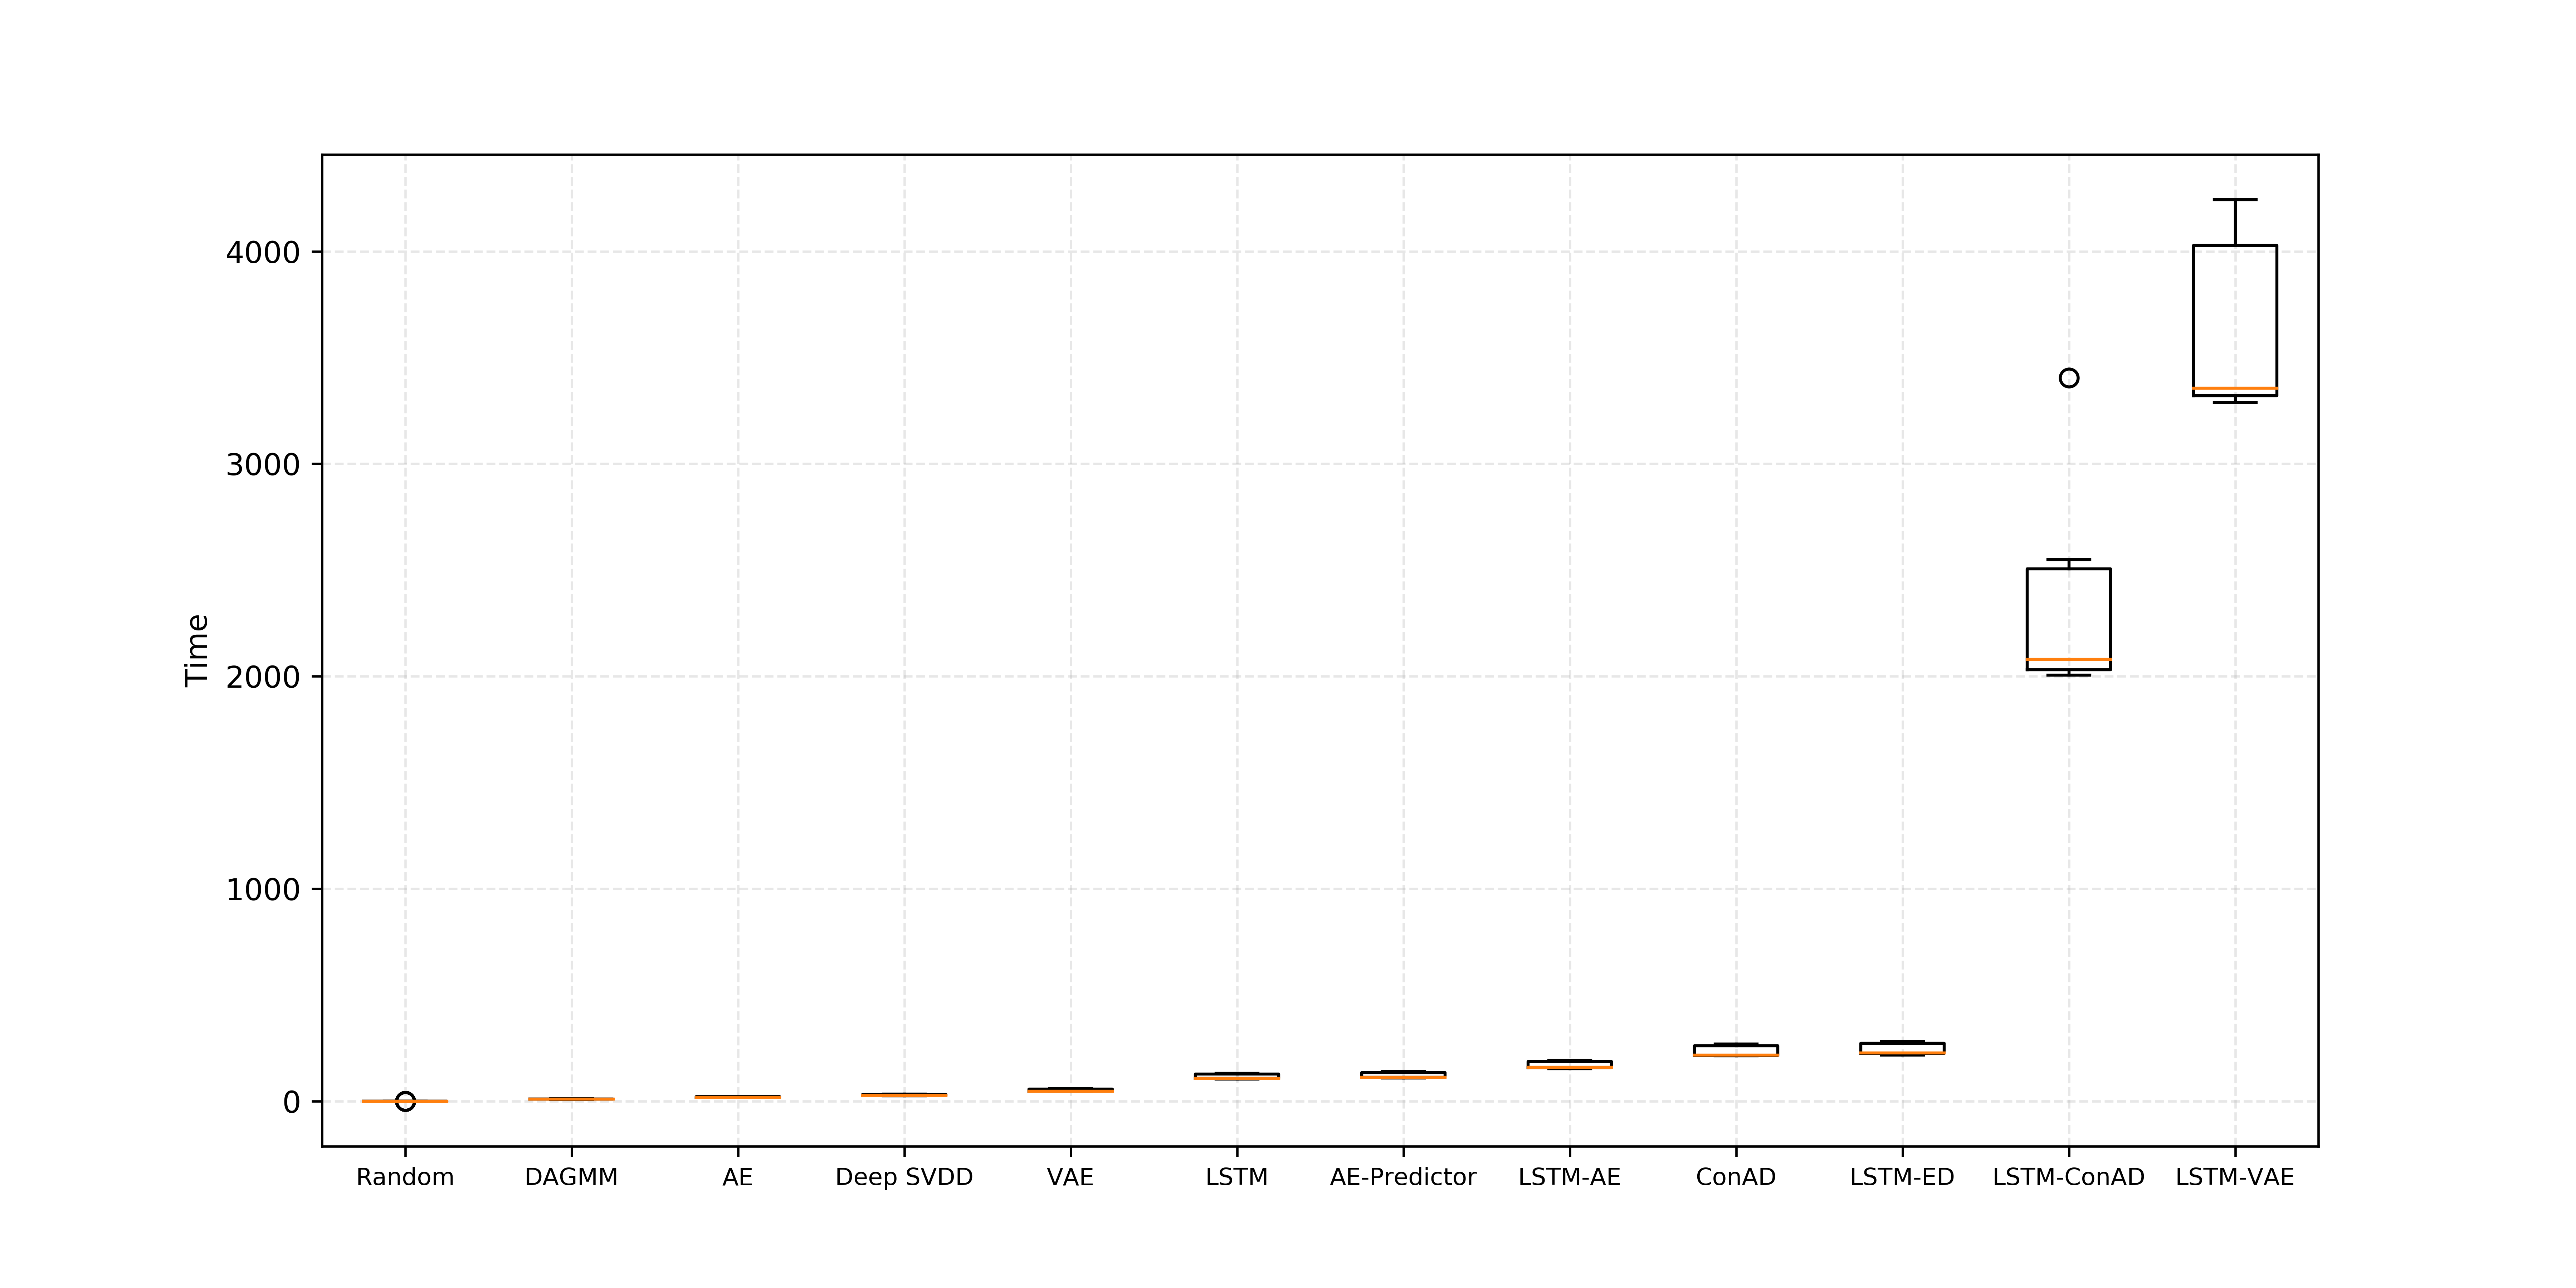
\includegraphics[width=\textwidth]{train_time.png}
  \caption{训练时间}
  \label{fig:train:time}
\end{figure}

图~\ref{fig:test:time}是所有算法的检测时间箱型图,可以看到LSTM-VAE因为使用了时序模型LSTM以及重构概率的计算要采样多次取平均,所以检测时间最长,而ConAD和LSTM-ConAD则是因为本身模型过于复杂在检测时花费时间相对较长,其他算法在检测时花费时间差距不大。

\begin{figure}[htbp]
  \centering
  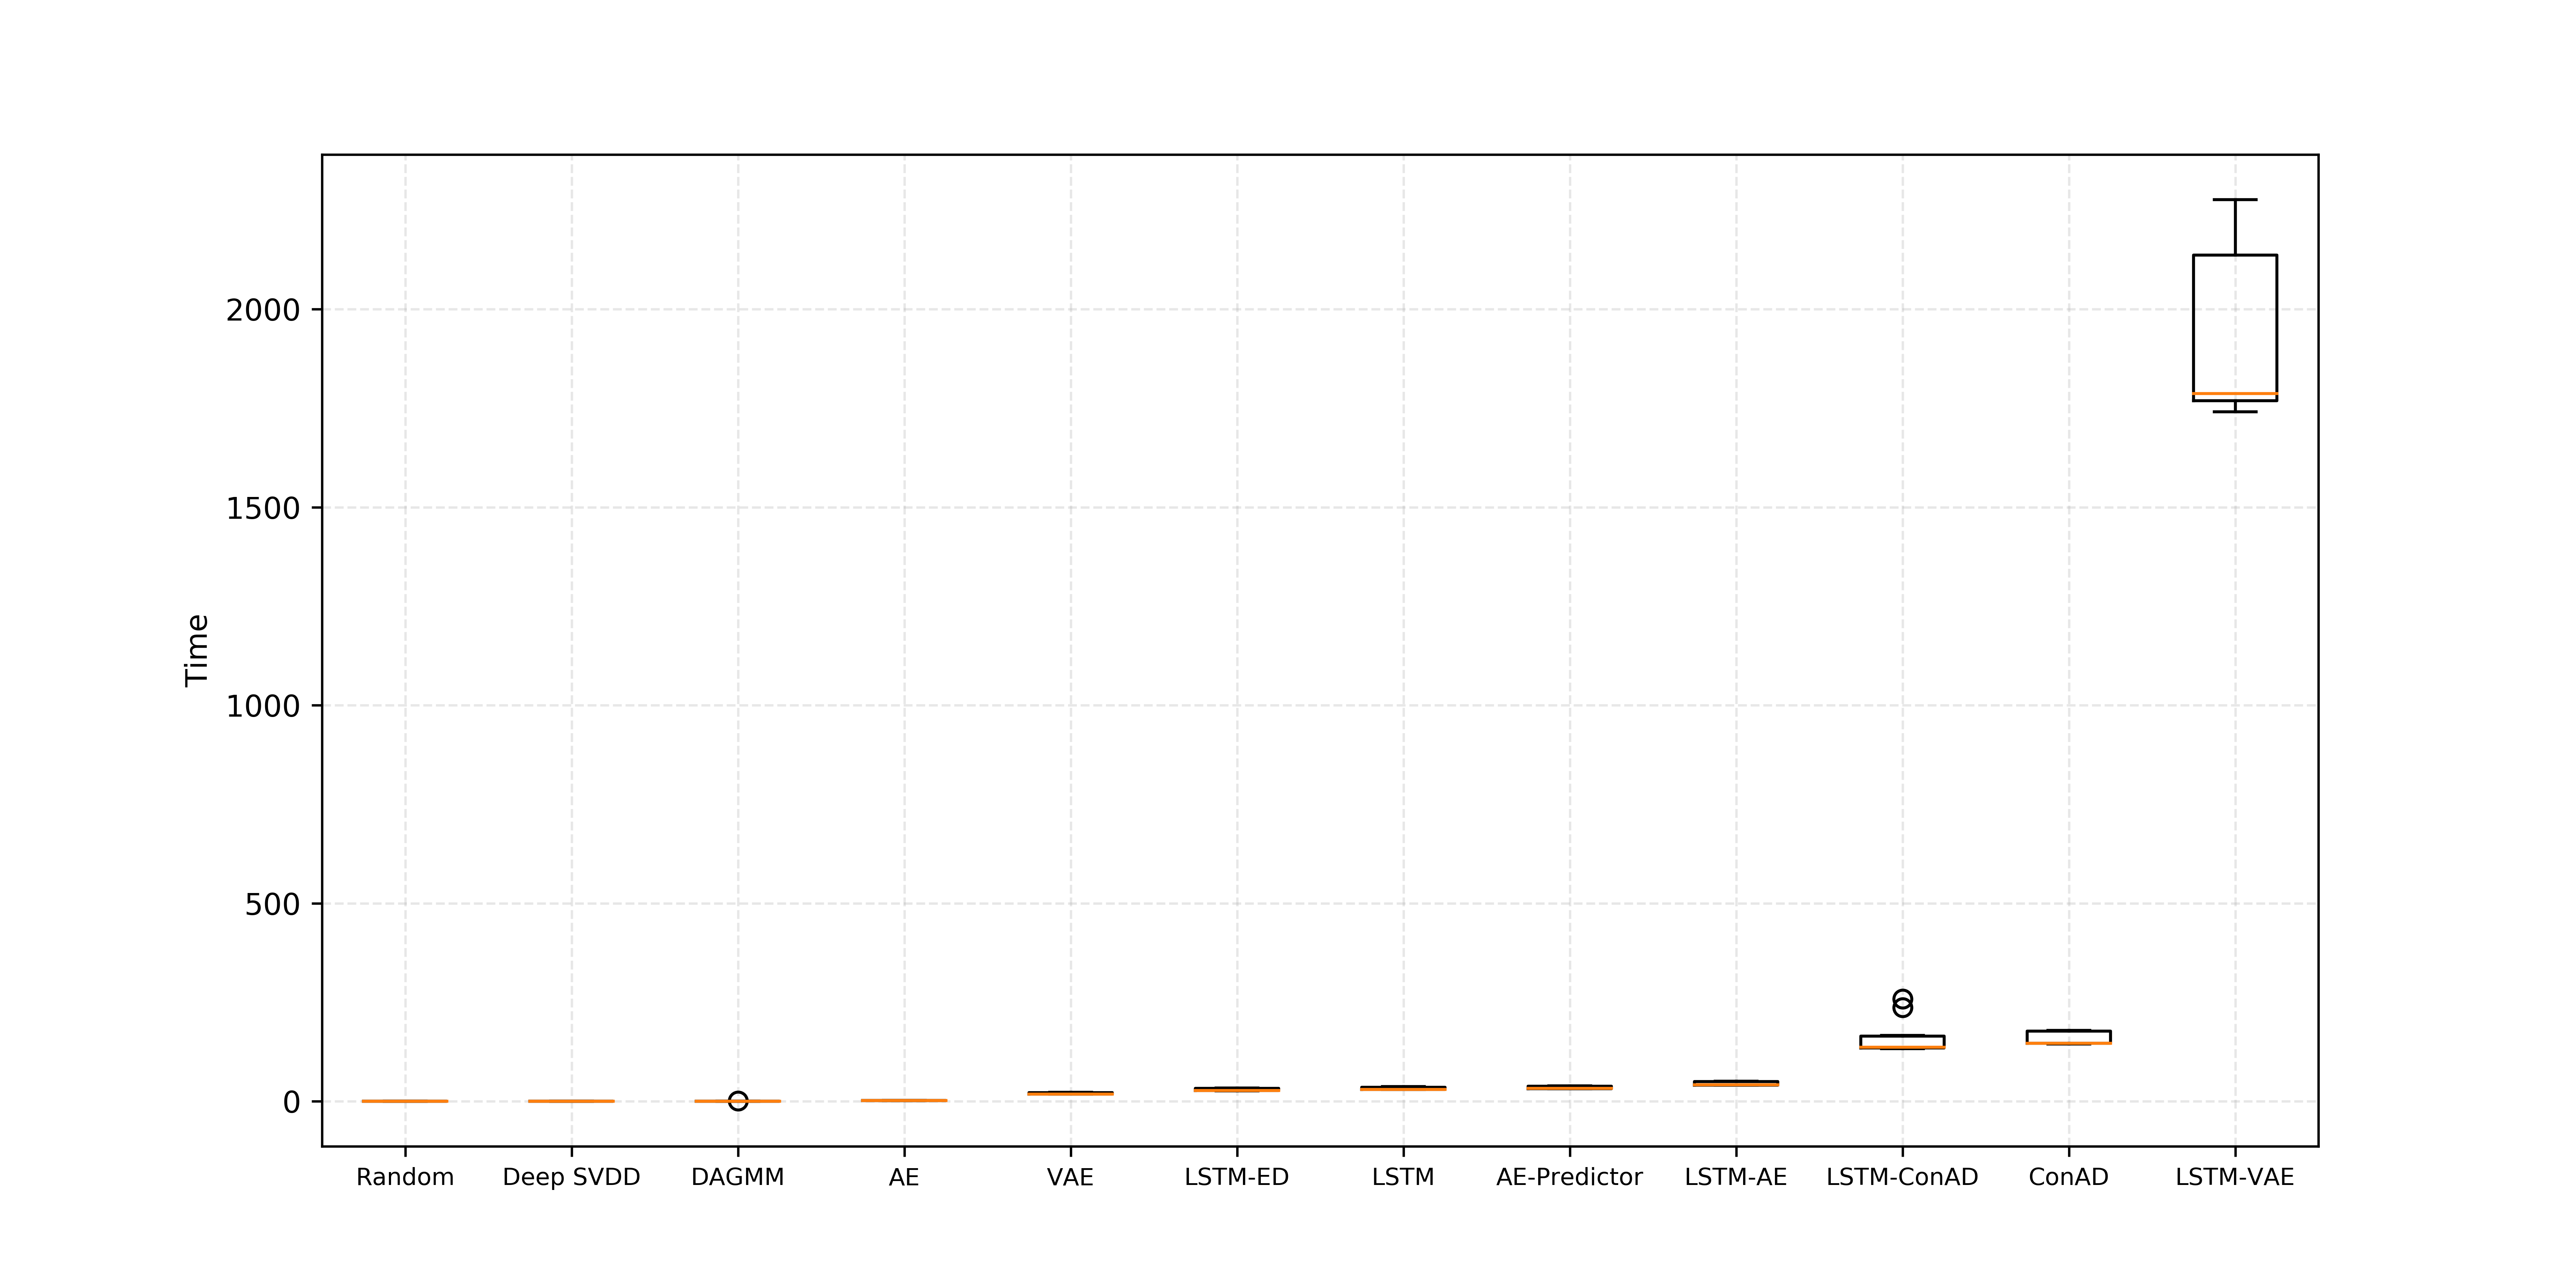
\includegraphics[width=\textwidth]{predict_time.png}
  \caption{检测时间}
  \label{fig:test:time}
\end{figure}

图~\ref{fig:pot:time}是所有算法用POT方法来确立阈值的耗时箱型图,虽然耗时的中位数很低,但是异常点很多,最坏情况下甚至达到了1000秒以上的耗时,而且稳定性较差,难以真正落地用到生产环境中去。

\begin{figure}[htbp]
  \centering
  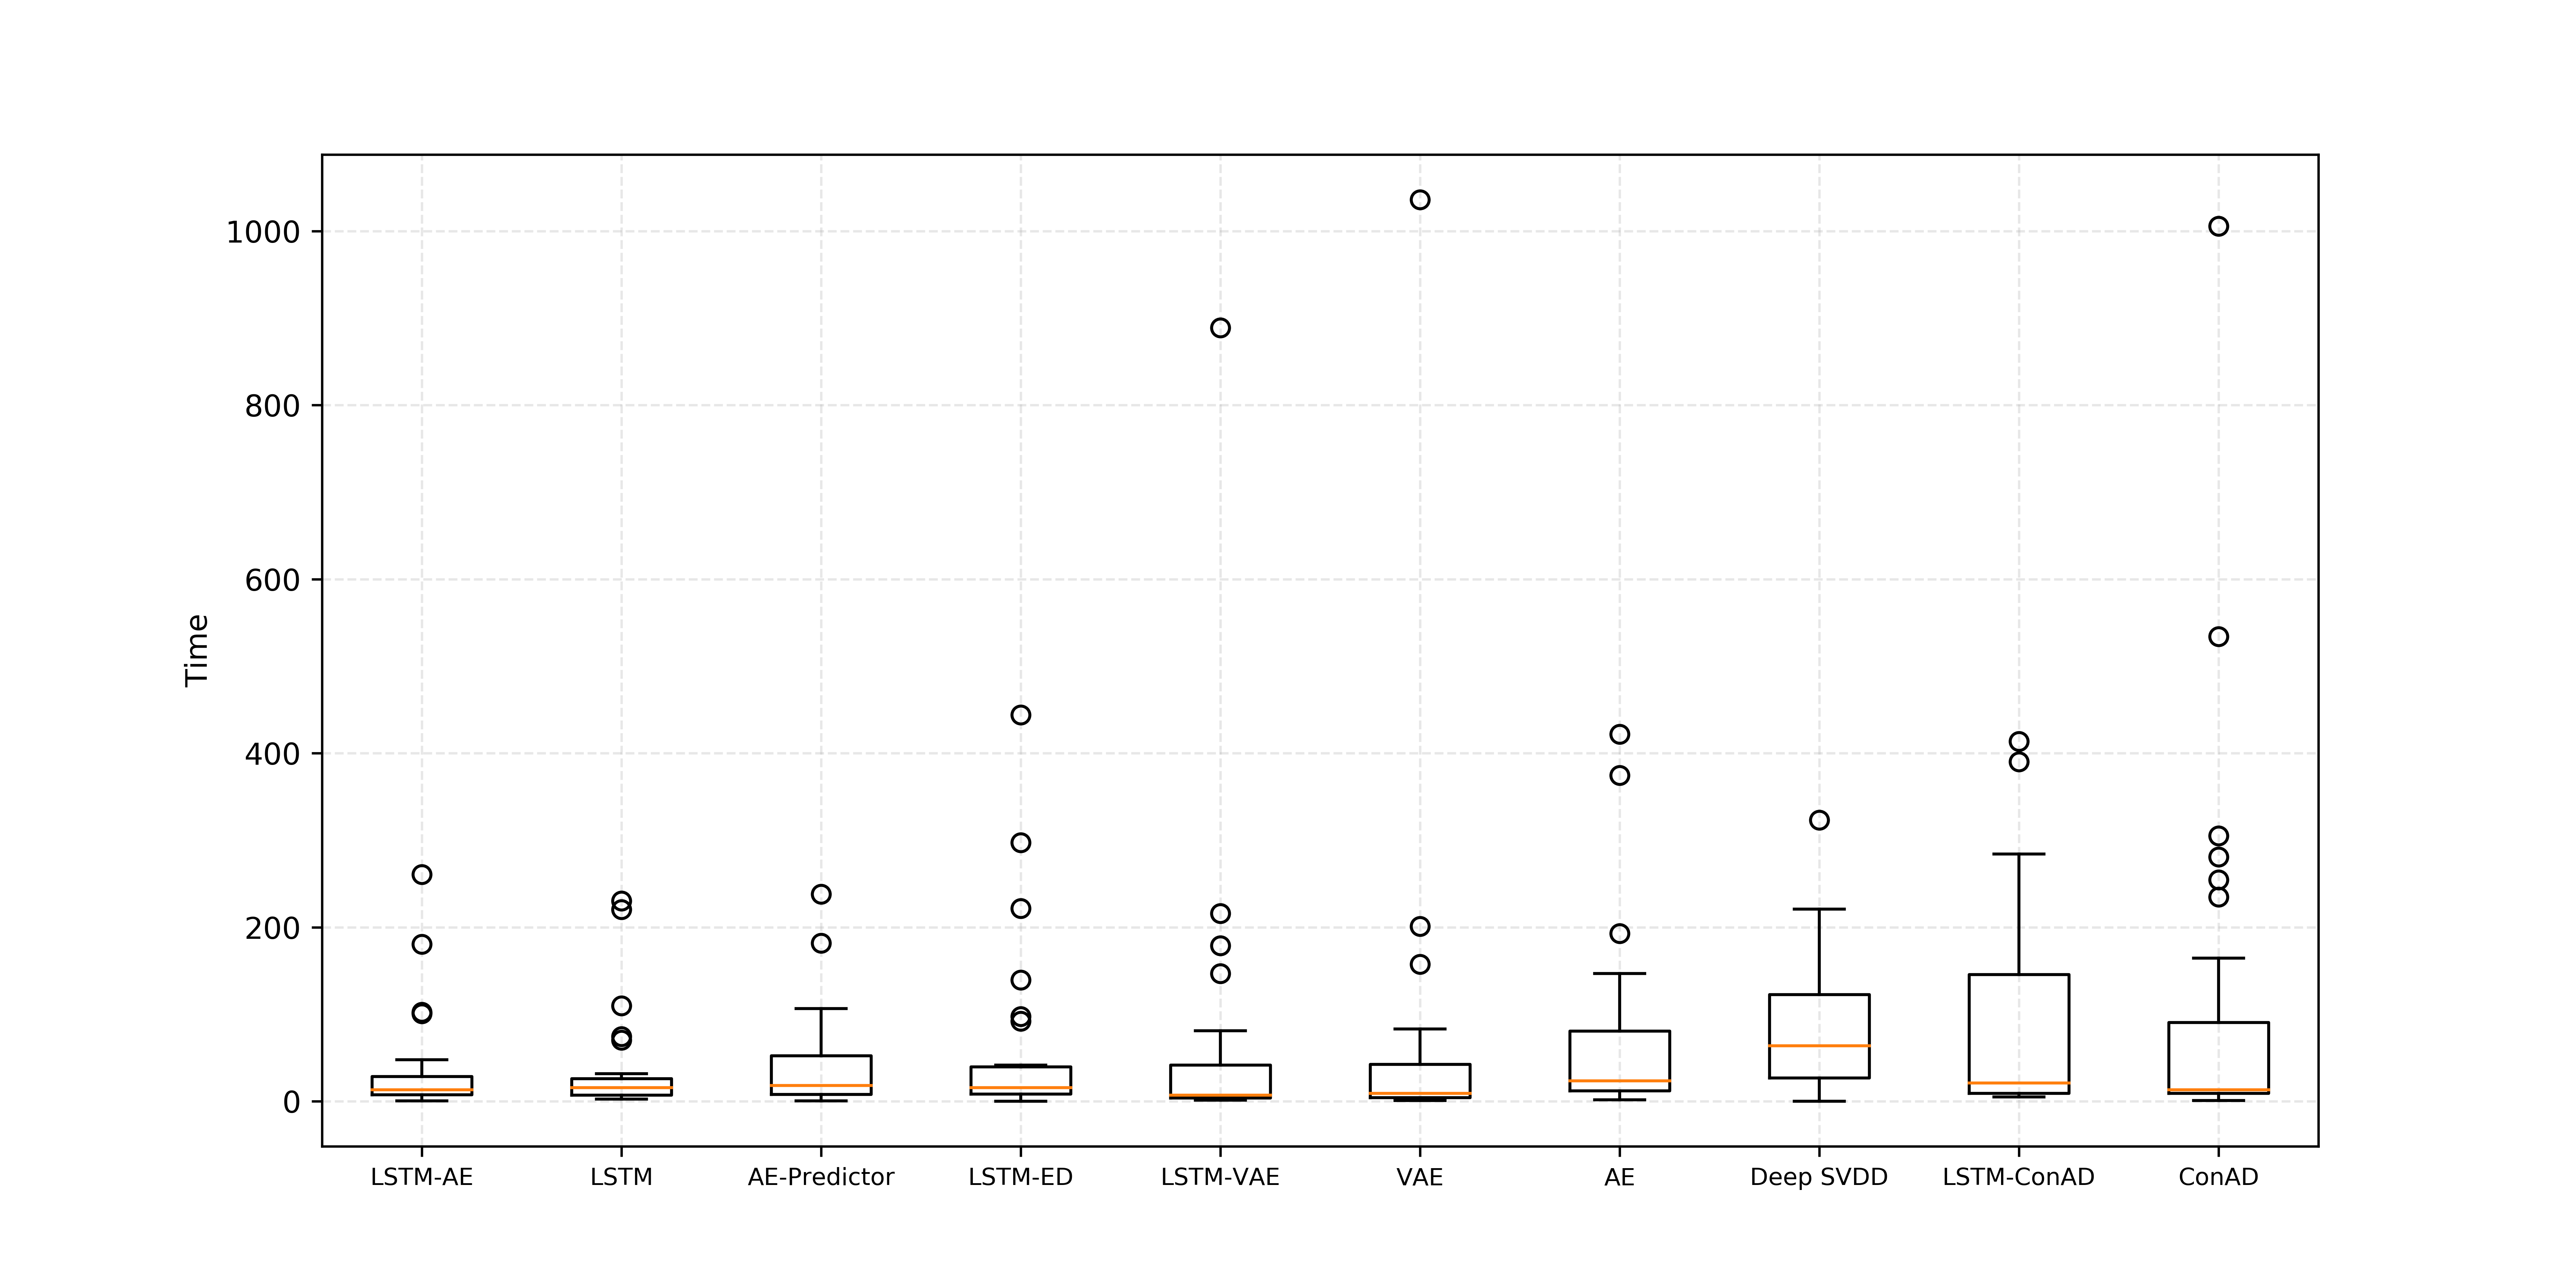
\includegraphics[width=\textwidth]{spot_time.png}
  \caption{POT方法评估时间}
  \label{fig:pot:time}
\end{figure}

图~\ref{fig:eval:time}则是所有算法用枚举所有阈值并选取最好的评估结果的耗时箱型图,从中看出这部分时间的消耗较为稳定且快速,而且不依赖于算法的效果。

\begin{figure}[htbp]
  \centering
  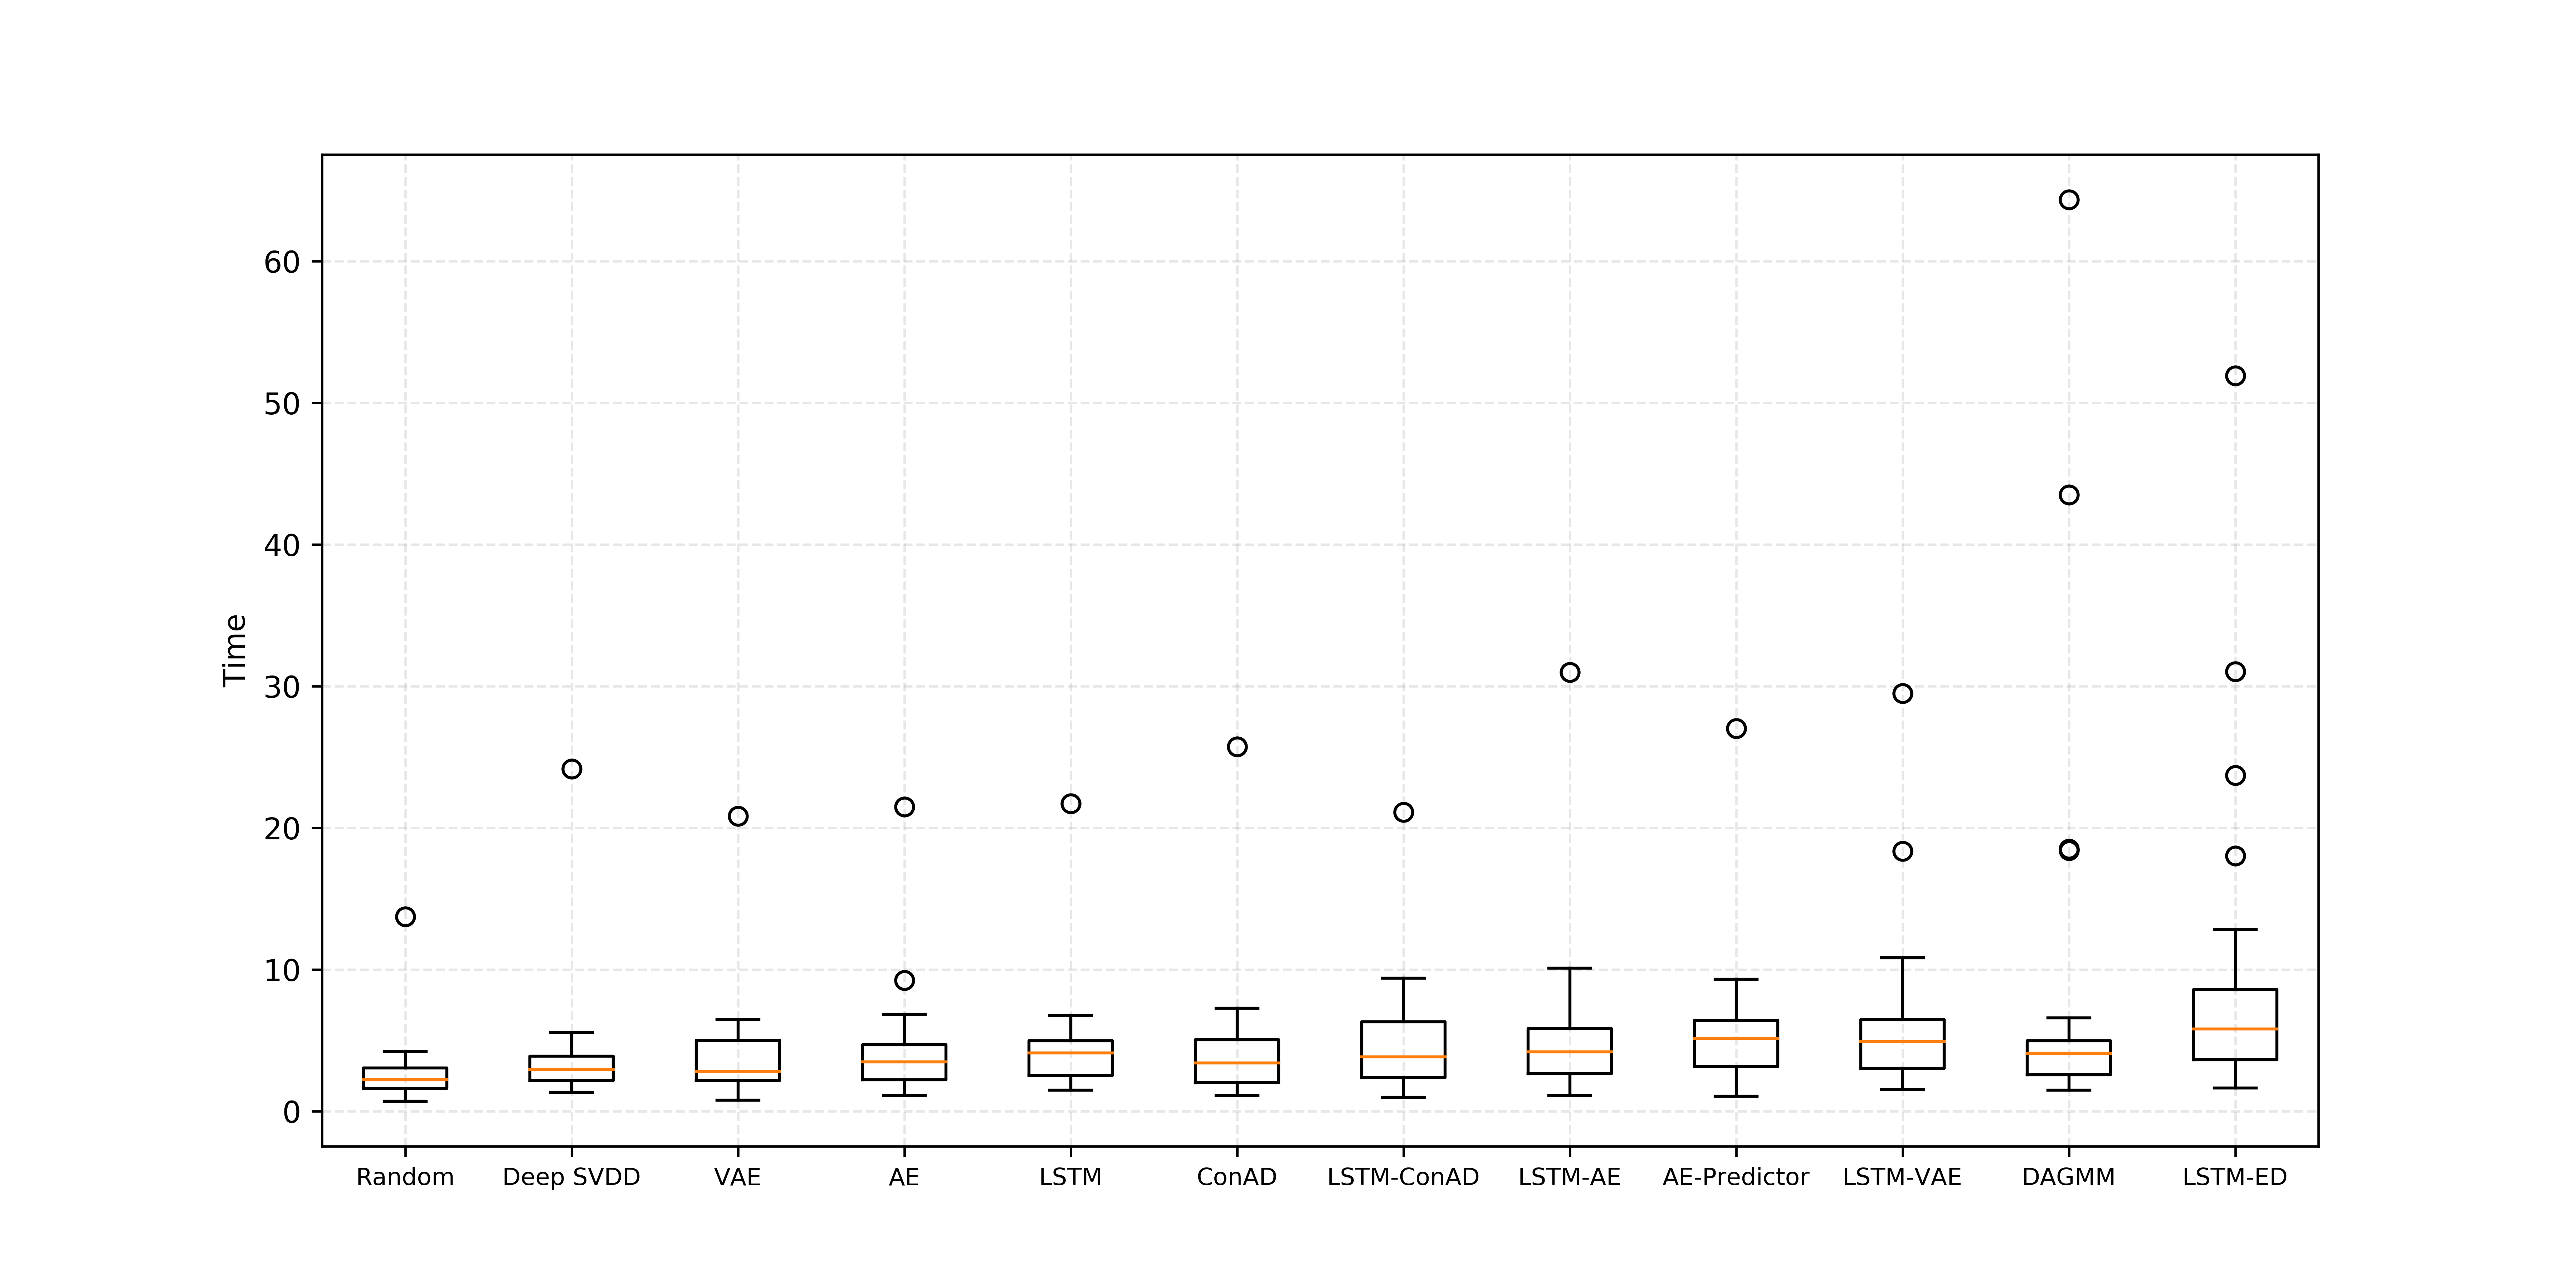
\includegraphics[width=\textwidth]{best_eval_time.png}
  \caption{枚举所有阈值评估时间}
  \label{fig:eval:time}
\end{figure}

\section{小结}
本章详细介绍了基于深度学习方法的时间序列异常检测框架各方面的设计思路,也对实现的算法在性能和效率上进行了综合的评估,将来如果有其他的算法也可以放到该框架内与其他算法进行比较。


